% !TEX root = ../main.tex

\section{Opdrachtbeschrijving}
\label{sec:opdrb}

Vul hier de \textcolor{blue}{opdrachtbeschrijving} in. 

tekst op \newline
twee lijnen \newline
Tekst in het vet \textbf{<h1>Welkom op mijn nginx webserver </h1>}\newline


%Alle code van deze opdracht is ook integraal te vinden op de volgende Github repository: %\newline
%\url{https://github.com/url}

%\subsection{bestandsnaam}
%\label{subsec:bestand}

%\begin{lstlisting}[language=sh, caption={ADD.vhd}, breakatwhitespace=false, %label={lst:add_tb}]

%\end{lstlisting}



\section{Opdracht Schema}
\label{sec:opdr-schema}

\begin{figure}[H]
  \centering
  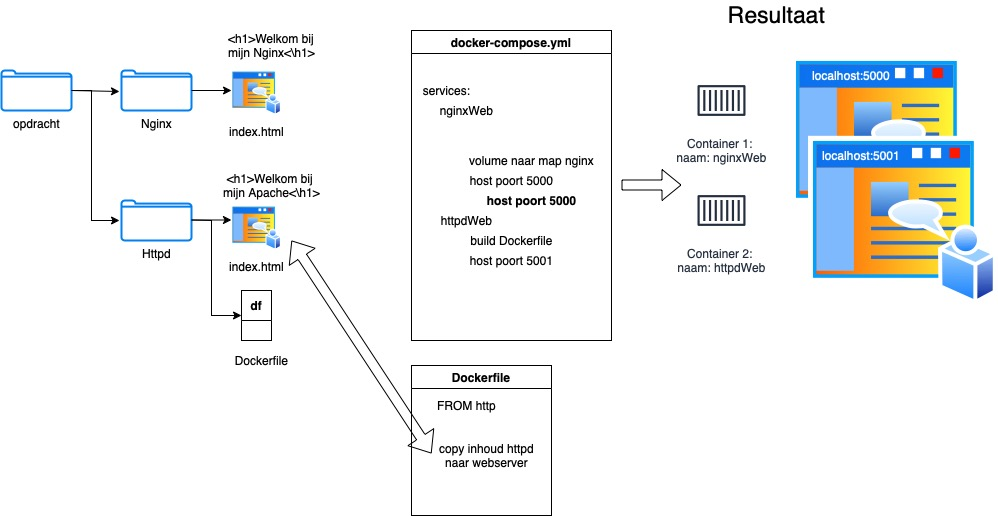
\includegraphics[width=1.3\textwidth, angle=90]{./lists/images/diagram.jpg}
  \caption{Opdracht diagram}
  \label{figure:opdr-diagram}
\end{figure}

